\chapter{Introduction to knot theory}

\section{Definition of a knot}

We normally conceive of knots as open strings with `knotted' parts in between. Given a knotted string with two `open' ends, we can simply pull one end of the string to untie it, in the usual way we untie a knot, by inserting an open end into the knotted region is a strategic manner and pulling it on the other side\footnote{There exists another way of unknotting an open knot, often used in magic tricks. One creates another knot using the unknotted portion of the string on one side of the knotted portion such that this new knot `cancels' the original knot. In mathematical terms, the new knot is constructed such that the \textit{connected sum} of the original knot and the new knot gives an unknot. We shall not deal with connected sums of knots in this thesis.}. This way, any knot with two open ends can be untied. But if have a knot in a closed loop, we won't be able to untie it unless we cut it. We want our notion of a knot to be invariant under `pulling'. Thus, we model our mathematical definition on closed loops instead of open. Refer to~\cref{fig:openclosedknots}.

\begin{figure}
    \centering
    \subcaptionbox{A knot with open ends}{
        \begin{tikzpicture}[scale=0.2]
            \begin{knot}[clip width = 8, consider self intersections = true, ignore endpoint intersections = false, use Hobby shortcut]
                \strand[thick, red] (-6,0)
                to (6,0)
                %to [out=0, in=135] (13,-2)
                to [out=0, in=180] (18, -4)
                to [out=0, in=-90] (21,0)
                to [out=90, in=0] (18,4)
                to [out=180, in=0] (9,-4)
                to [out=180, in=-90] (6,0)
                to [out=90, in=180] (9,4)
                to [out=0, in=180] (21,0)
                to (33,0);
                \flipcrossings{1,2,4,5,6,7,8,9}
            \end{knot}
        \end{tikzpicture}}\par\bigskip
    \subcaptionbox{A knot with closed ends}{
        \begin{tikzpicture}[scale=0.2]
            \begin{knot}[clip width = 8, consider self intersections = true, ignore endpoint intersections = false, use Hobby shortcut]
                \strand[thick, red] (2,0) to (6,0)
                to [out=0, in=180] (18, -4)
                to [out=0, in=-90] (21,0)
                to [out=90, in=0] (18,4)
                to [out=180, in=0] (9,-4)
                to [out=180, in=-90] (6,0)
                to [out=90, in=180] (9,4)
                to [out=0, in=180] (21,0)
                to (25,0);
                \flipcrossings{4,5,7,8,9,11,12}
            \end{knot}
            \draw[thick, red, rounded corners] (2,0) -- (1,0) -- (0,-1) -- (0,-5) -- (1,-6) -- (26,-6) -- (27,-5) -- (27,-1) -- (26,0) -- (25,0);
%             \draw[thick, red, rounded corners=9] (1,-6) -- (0,-6) -- (0,0) -- (1,0);
        \end{tikzpicture}}
    \caption{Projections of a knot on a plane}
    \label{fig:openclosedknots}
\end{figure}

\begin{defn}[Knot]
    A knot \(K\) is an embedding of \(\sone\) in \(\rthree\).
\end{defn}

\begin{figure}
    \centering
    \begin{tikzpicture}[scale=0.2]
        \begin{knot}[clip width = 8, consider self intersections = true, ignore endpoint intersections = false, use Hobby shortcut]
            \strand[thick, red] (1,0)
            to (6,0)
            to [out=0, in=180] (18, -4)
            to [out=0, in=-90] (21,0)
            to [out=90, in=0] (18,4)
            to [out=180, in=0] (9,-4)
            to [out=180, in=-90] (6,0)
            to [out=90, in=180] (9,4)
            to [out=0, in=180] (21,0)
            to (22.5,0);
            \flipcrossings{1,2,4,5,6,7,8,9}
        \end{knot}
            \begin{scope}[xshift=23cm, scale=0.6]
                \begin{knot}[clip width = 6, consider self intersections = true, ignore endpoint intersections = false, use Hobby shortcut]
                    \strand[thick, red] (-2,0)
                    to (6,0)
                    to [out=0, in=180] (18, -4)
                    to [out=0, in=-90] (21,0)
                    to [out=90, in=0] (18,4)
                    to [out=180, in=0] (9,-4)
                    to [out=180, in=-90] (6,0)
                    to [out=90, in=180] (9,4)
                    to [out=0, in=180] (21,0)
                    to (23,0);
                    \flipcrossings{1,2,4,5,6,7,8,9}
                \end{knot}
            \end{scope}
                \begin{scope}[xshift=37cm, scale=0.35]
                    \begin{knot}[clip radius =3pt, clip width = 3, consider self intersections = true, ignore endpoint intersections = false, use Hobby shortcut]
                        \strand[thick, red] (-2,0)
                        to (6,0)
                        to [out=0, in=180] (18, -4)
                        to [out=0, in=-90] (21,0)
                        to [out=90, in=0] (18,4)
                        to [out=180, in=0] (9,-4)
                        to [out=180, in=-90] (6,0)
                        to [out=90, in=180] (9,4)
                        to [out=0, in=180] (21,0)
                        to (23,0);
                        \flipcrossings{1,2,4,5,6,7,8,9}
                    \end{knot}
                \end{scope}
                    \begin{scope}[xshift=45cm, scale=0.2]
                        \begin{knot}[clip radius =3pt, clip width = 1.7, consider self intersections = true, ignore endpoint intersections = false, use Hobby shortcut]
                            \strand[thick, red] (-2,0)
                            to (6,0)
                            to [out=0, in=180] (18, -4)
                            to [out=0, in=-90] (21,0)
                            to [out=90, in=0] (18,4)
                            to [out=180, in=0] (9,-4)
                            to [out=180, in=-90] (6,0)
                            to [out=90, in=180] (9,4)
                            to [out=0, in=180] (21,0)
                            to (22,0);
                            \strand [thick, red, only when rendering/.style={densely dotted}] (22,0) to (46,0);
                            \flipcrossings{1,2,4,5,6,7,8,9}
                        \end{knot}
                    \end{scope}
        \draw[thick, red, rounded corners] (1,0) to (0,0) to (0,-6) to (55,-6) to (55,0) to (53,0);
        \node (p) at (53,1.5) {\(p\)};
        \filldraw[black] (53,0) circle (5pt);
    \end{tikzpicture}
    \caption{A wild knot. The knot is wild only at the point \(p\).}
    \label{fig:wildknot}
\end{figure}

Although one can talk about embeddings of higher dimensional `circles' in higher dimensional spaces, we restrict ourselves to knots in the three dimensional space. The above definition turns out out to be too general for our purposes. It takes into consideration certain pathological knots known as \textit{wild knots}. Although wild knots are an object of study, we shall not be dealing with them in this thesis due to their pathological nature. \Cref{fig:wildknot} shows an example of a wild knot. A section of the knot is scaled down by a factor and then joined on one side of the previous section. If one repeats this process infinitely, the resulting curve formed by appending sections eventually converges to a point, provided that the scaling down is fast enough. We can join the convergence (limit) point to a an end-section on the other side to get wild knot. This knot is continuous everywhere, including the limit point. The behaviour of the knot at the limit point is different from the other points. Three common ways exist to exclude such behaviour by demanding extra conditions.
\begin{enumerate}
    \item Differentiability.

    We can demand all knots to be differentiable at all points. We can verify visually that all the points, except the limit point of the wild knot are differentiable, or can be made (isotoped) differentiable. The derivative must necessarily change within a section. As the size of the section decreases, the derivative changes more rapidly. In a scaled down section, all the values which the derivative took in the previous section. As we approach the sections near the limit point, the derivative function must attain all the values it did before, but it must do so in a more rapid manner. At the limit point, the derivative shall cease to exist by the virtue of `changing too rapidly'. Demanding differentiability forcibly removes the offending limit point. The wildness is due to the limit point. Along with differentiability, we can demand \(\symup{C}^r\) smoothness or \(\symup{C}^\infty\) smoothness as well.

    But this condition comes with a problem as well, namely we cannot use polygons for describing knots.
    \item Piecewise linearity.

    We can demand all the edges of a knot to be piecewise linear with finitely many edges. Our knot shall be a polynomial (with finitely many edges) in that case. Infinitely (countably) many sections in a wild knot shall mean infinitely many edges (of decreasing length), which is not allowed. Thus, this condition excludes wild knots.
    \item Local flatness.
\end{enumerate}
In this thesis, we shall take the third route following Cromwell~\cite[chp.~1]{cromwell}. Local flatness is a topological condition unlike other other two. If we consider a local neighbourhood around each point of the knot, except the limit point, then we see visually see that we can always find a small enough local neighbourhood around each such point such that the strand is not `knotted' in that neighbourhood. At the limit point, no matter how small a neighbourhood we take, the strand shall always be `knotted'. We enforce this `local unknottedness' condition by demanding local flatness. Let \(p\) be a point in a knot \(K\), \(\symup{B}(\symup{O}, 1)\) be the unit ball centered at origin \(\symup{O}\) and \(d\) be a diameter of \(\symup{B}(\symup{O}, 1)\).
\begin{defn}[Local flatness]
    The point \(p\) is said to be locally flat if there exists a neighbourhood \(U \ni p\) such that the pair \((U, U \cap K)\) is homeomorphic to \((\symup{B}(\symup{O}, 1), d)\).

    A knot is said to be locally flat if each point in that knot is locally flat. A point that is not locally flat is called wild, and a knot is wild if any of its points are wild.
\end{defn}

Consider a spherical neighbourhood around a locally flat point. There exists a radius such that for all neighbourhoods less than this radius, the boundary of the neighbourhood intersects the strand in exactly two points. This is not possible at the limit point in wild knot figure.

\begin{defn}[Tame knots]
    A knot is said to be tame if all its points are locally flat.
\end{defn}

\section{Distinguishing knots}

Any two homeomorphisms of the circle are homeomorphic to the circle and to each other, since being homeomorphic is an equivalence relation. But this means that all knots are homeomorphic to each other. Clearly, homeomorphism is not the correct notion to distinguish knots. When we mean that two knots are distinct, we mean that if we create a physical model of those knots, we cannot `physically deform' one knot into another. \textit{Cutting a knot is not allowed.} One might think that homotopy or isotopy are what we need, but it turns out that the notion of \textit{ambient isotopy} is the correct one.

\begin{defn}[Homotopy]
    A homotopy of a space \(X \subset \rthree\) is a continuous map \(h \colon X \times [0, 1] \rightarrow \rthree\).

    The restriction of \(h\) to level \(t \in [0, 1]\) is \(h_t \colon X \times \{t\} \rightarrow \rthree\). \(h_0\) must be the identity map.
\end{defn}
Note that the continuity of \(h\) implies the continuity of \(h_t\) for all \(t \in [0,1]\). The converse is not true. Insert example here. Homotopy allows a curve to pass through itself. All knots are thus homotopic to the trivial knot. If we do not allow a curve to pass through itself, i.e.\@ if we demand injectivity for each \(h_t\), then we get what is known as an isotopy. But isotopy is not useful for distinguishing knots as well, due to bachelors' unknotting. All tame knots, or more generally, all knots with a tame arc turn out to be isotopic to the trivial knot. It is an open problem if all knots are isotopic to the trivial knot~\cite{ancel, shijie}. In addition, it is not known as well if a knot known as the Bing sling, which is wild \textit{at all points} is isotopic to the trivial knot~\cite{ancel, shijie}.
\begin{prop}[Bachelors' unknotting]
    Every knot with a tame arc is isotopic to the unknot.
\end{prop}
\begin{proof}
    \begin{figure}
        \centering
        \subcaptionbox{\(i_0 (K)\)}{
            \begin{tikzpicture}[scale=0.2]
                \begin{knot}[clip width = 10, consider self intersections = true, ignore endpoint intersections = false, use Hobby shortcut]
                    \strand[thick, red] (1,0) to (6,0)
                    to [out=0, in=180] (18, -4)
                    to [out=0, in=-90] (21,0)
                    to [out=90, in=0] (18,4)
                    to [out=180, in=0] (9,-4)
                    to [out=180, in=-90] (6,0)
                    to [out=90, in=180] (9,4)
                    to [out=0, in=180] (21,0)
                    to (26,0);
                    \flipcrossings{4,5,7,8,9,11,12}
                \end{knot}
                \draw[thick, red, rounded corners] (26,0) -- (27,0) -- (27,-6) -- (0,-6) -- (0,0) -- (1,0);
                \filldraw[black] (13.5,-6) circle (5pt) node[anchor=north, yshift=-0.3cm]{\(p\)};
                \draw[densely dashed, line width=0.6pt, rounded corners, closed] (3,-1) to (3,1) to (-1,1) to (-1,-7) to (28,-7) to (28,1) to (24,1) to (24,-1) to (26,-1) to (26,-5) to (1,-5) to (1,-1) -- cycle;
                \node at (26.4,2.5) {\(U_p\)};
            \end{tikzpicture}}
        \subcaptionbox{\(i_{0.3} (K)\)}{
            \begin{tikzpicture}[scale=0.2]
                \begin{scope}[xshift=4cm, scale=0.7]
                    \begin{knot}[clip width = 7, consider self intersections = true, ignore endpoint intersections = false, use Hobby shortcut]
                        \strand[thick, red] (0,0) to (6,0)
                        to [out=0, in=180] (18, -4)
                        to [out=0, in=-90] (21,0)
                        to [out=90, in=0] (18,4)
                        to [out=180, in=0] (9,-4)
                        to [out=180, in=-90] (6,0)
                        to [out=90, in=180] (9,4)
                        to [out=0, in=180] (21,0)
                        to (27,0);
                        \flipcrossings{4,5,7,8,9,11,12}
                    \end{knot}
                \end{scope}
                \draw[thick, red, rounded corners, rounded corners] (22,0) to (27,0) to (27,-6) to (0,-6) -- (0,0) -- (5,0);
                \filldraw[black] (13.5,-6) circle (5pt) node[anchor=north, yshift=-0.3cm]{\(p\)};
                \draw[densely dashed, line width=0.6pt, rounded corners] (3,-1) to (3,1) to (-1,1) to (-1,-7) to (28,-7) to (28,1) to (24,1) to (24,-1) to (26,-1) to (26,-5) to (1,-5) to (1,-1) -- cycle;
                \node at (26.4,2.5) {\(U_p\)};
            \end{tikzpicture}}
        \subcaptionbox{\(i_{0.6} (K)\)}{
            \begin{tikzpicture}[scale=0.2]
                \begin{scope}[xshift=8cm, scale=0.4]
                    \begin{knot}[clip radius = 2pt, clip width = 4, consider self intersections = true, ignore endpoint intersections = false, use Hobby shortcut]
                        \strand[thick, red] (0,0) to (6,0)
                        to [out=0, in=180] (18, -4)
                        to [out=0, in=-90] (21,0)
                        to [out=90, in=0] (18,4)
                        to [out=180, in=0] (9,-4)
                        to [out=180, in=-90] (6,0)
                        to [out=90, in=180] (9,4)
                        to [out=0, in=180] (21,0)
                        to (30,0);
                        \flipcrossings{4,5,7,8,9,11,12}
                    \end{knot}
                \end{scope}
                \draw[thick, red, rounded corners] (19,0) to (27,0) to (27,-6) to (0,-6) to (0,-6) -- (0,0) -- (8.1,0);
                \filldraw[black] (13.5,-6) circle (5pt) node[anchor=north, yshift=-0.3cm]{\(p\)};
                \draw[densely dashed, line width=0.6pt, rounded corners] (3,-1) to (3,1) to (-1,1) to (-1,-7) to (28,-7) to (28,1) to (24,1) to (24,-1) to (26,-1) to (26,-5) to (1,-5) to (1,-1)  -- cycle;
                \node at (26.4,2.5) {\(U_p\)};
            \end{tikzpicture}}
        \subcaptionbox{\(i_1 (K)\)}{
            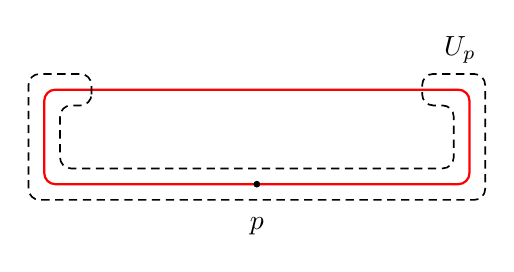
\begin{tikzpicture}[scale=0.2]
                \draw[thick, red, rounded corners] (22,0) to (27,0) to (27,-6) to (0,-6) -- (0,0) -- (22,0);
                \filldraw[black] (13.5,-6) circle (5pt) node[anchor=north, yshift=-0.3cm]{\(p\)};
                \draw[densely dashed, line width=0.6pt, rounded corners] (3,-1) to (3,1) to (-1,1) to (-1,-7) to (28,-7) to (28,1) to (24,1) to (24,-1) to (26,-1) to (26,-5) to (1,-5) to (1,-1) -- cycle;
                \node at (26.4,2.5) {\(U_p\)};
            \end{tikzpicture}}
        \caption{Bachelors' unknotting demonstrating the isotopy equivalence of a knot with tame arc to the trivial knot. Here we have chosen the point \(r\) (not shown in the figure) to be the midpoint of the knotted region. \(f(a)\) and \(f(b)\) are the intersections of the knot \(K\), represented by the thick red line, with \(U_p\), shown using densely dashed lines. Note that \(f(a)\), \(r\) and \(f(b)\) are collinear in this case. The entirety of the knot is tame in this case, but we only require tameness in the chosen region of \(U_p \cap K\).}
        \label{fig:bachelor}
    \end{figure}

    Refer to \cref{fig:bachelor}. Let \(K \subset \rthree\) be a knot with a tame arc.

    Let \(p \in K\) in a tame arc of the knot. Since the knot is locally flat on the arc, by the definition of tameness, we take a ball \(U_p \subset \rthree\) of radius \(\varepsilon\) around the point \(p\) such that the pair \(U_p, U_p \cap K\) is homeomorphic to \((\symup{B}, \symup{d})\), where \(\symup{B}\) is the unit ball in \(\rthree\) centered at the origin and \(\symup{d}\) is the diameter of \(\symup{B}\) along the \(x\)-axis. We choose a parametrization \(f \colon [0, 2\pii) \rightarrow K\) of the knot such that \(f([a, b]) = K - (U_p \cap K) \), where \([a, b] \subset [0, 2\pii)\).

    Let \(r \in \rthree\) be a point outside \(U_p\). Now consider the function \(i_t \colon K \rightarrow \rthree\), defined for each \(t \in [0, 1]\) as follows.
    Let \[\phi_t(a) \coloneq t\left(\frac{a+b}{2}\right) + (1-t)a\] be a family of functions for all \(t \in [0,1]\).
    \begin{enumerate}
        \item If \(f(x) \in U_p\), then \[i_t(f(x)) = f(x).\]
        \item If \(\displaystyle x \in [a, \phi_t(a))\), then \[ i_t(f(x)) = f(a) + \frac{\norm{f(a) - f(\phi_t(a))}}{\norm{a - \phi_t(a)}}(x - a)(r - f(a)).\]
        \item If \(x \in [\phi_t(a), \phi_t(b)]\), then \[i_t(f(x)) = tr + (1-t)f(x).\]
        \item If \(\displaystyle x \in (\phi_t(b), b]\), then \[ i_t(f(x)) = f(b) + \frac{\norm{f(b) - f(\phi_t(b))}}{\norm{b - \phi_t(b)}}(b - x)(r - f(b)).\]
    \end{enumerate}
    Let \(i \colon [0, 1] \times K \rightarrow \rthree\) be a function defined by \(i(t, f(x)) \coloneq i_t (f(x))\).

    \(i\) is defined such that the part inside \(U_p\) is kept unchanged for all \(t\). For \(t =0\), \(i\) does not deform the knot at all. For \(t \in (0, 1)\), the knotted part (in \(\rthree\)) shrinks and the interval in the domain \([a,b]\) which maps to the knotted part also shrinks to \([\phi_t(a), \phi_t(b)]\). This shrinkage of the domain happens linearly with \(t\). Refer to \cref{fig:graphbachelor}. All points of the knotted part trace a straight line as they travel under isotopy from their original position to \(r\). Eventually, the knotted part ceases to exist at \(t = 1\) and a single point of the domain, namely, \((a + b)/2\) maps to \(r\).

    \begin{figure}
        \centering
        \begin{tikzpicture}[scale=1.4]
            \draw[thick, blue, <->] (0,4.5) node[anchor=south]{\(x\)} -- (0,0) -- (5,0);
            \draw[line width=0.6pt, black] (-2.5pt,4) node[anchor=east, black]{\(2\pii\)} -- (2.5pt,4);
            \node at (0,-0.2) {\(0\)};
            \node at (4,-0.2) {\(1\)};

            \draw[black, dotted, line width=0.6pt] (0,2) node[anchor=east, black]{\((a+b)/2\)} -- (4,2);
            \draw[black, dotted, line width=0.6pt] (2,0) -- (2,4);
            \draw[black, densely dashed, line width=0.7pt] (2,1.5) -- (0,1.5) node[anchor=east, black]{\(\phi_t(a)\)};
            \draw[black, densely dashed, line width=0.7pt] (2,2.5) -- (0,2.5) node[anchor=east, black]{\(\phi_t(b)\)};
%             \node at (-0.36,1.5) {\(\phi_t(a)\)};
%             \node at (-0.36,2.5) {\(\phi_t(b)\)};
%             \node at (-0.6,1.98) {\((a+b)/2\)};
            \node at (2,-0.2) {\(t\)};
            \draw[thick, red] (0,1) node[anchor=east, black]{\(a\)} -- (4,2) -- (0,3) node[anchor=east, black]{\(b\)};
        \end{tikzpicture}
        \caption{Illustration of shrinkage of domain with respect to \(t\). For all \(t \in [0,1]\), the interval \([\phi_t(a), \phi_t(b)] \in [0,2\pii)\) maps to the shrunk `knotted' part. The images of \([a,\phi_t(a)]\) and \([\phi_t(b),b]\) map to the straight lines which connect \(f(a)\) to \(i_t(f(\phi_t(a)))\) and \(i_t(f(\phi_t(b)))\) to \(f(b)\) respectively.}
        \label{fig:graphbachelor}
    \end{figure}

    In the end, we get a figure consisting of two straight lines meeting at \(r\), and \(U_p \cap K\), the original part of the knot inside \(U_p\). The other endpoints of these lines are \(f(a)\) and \(f(b)\). \(U_p \cap K\) is isotopic to the line joining \(f(a)\) and \(f(b)\). Thus, we get a triangle with points \(r\), \(f(a)\) and \(f(b)\) and we any that any triangle in \(\rthree\) is isotopic to \(\sone\).

    We now prove that \(i\) is continuous. We know that both \(i_t\) and \(i_x\) are continuous and injective for all \(t \in [0, 1]\) and \(x \in [0, 2\pii)\) respectively, where \(i_x\) is defined to be the restriction of \(i\) for a particular \(x\). We also see that \(i_t\) is linear in \(x\). A function continuous in one argument and linear in the other is continuous in the product topology. We thus have an isotopy which sends a knot with a tame arc to \(\sone\).
\end{proof}

\begin{remark}
    It should be noted that the isotopy that we have constructed does not shrink \(K - (U_p \cap K)\) uniformly. Parts of the strand closer to the point \(r\) are shrunk more than the parts further away. Also, not all parts move at a uniform rate towards \(r\). Parts closer to \(r\) move slower than the parts further.%\footnote{The knotted parts are scaled uniformly though in \cref{fig:bachelor} due to the ease of drawing such a figure.}.
\end{remark}


In the above considered isotopy, we isotoped the set \(X = K\). Instead, we take \(X\) to be the entire space \(\rthree\), or a bounded set which completely covers the knot, then we get the notion of ambient isotopy. This modification ensures that the surrounding space is isotoped as well as we isotope the knot. The knot is a curve which has no volume. If we try bachelors' unknotting on the surrounding space as well, we observe that the surrounding space, which has a finite, non-zero volume cannot shrink to a set of zero volume under isotopy. This finally leads us to the equivalence relation induced by ambient isotopy.

\begin{remark}
    Unless mentioned otherwise, we shall always consider our knots to be tame from now on.
\end{remark}

\begin{defn}[Knot equivalence]
    Two knots \(K_1\) and \(K_2\) are said to be ambient isotopic if there exists an isotopy \(I \colon \rthree \times [0,1] \rightarrow \rthree\) such that \(I(K_1,0) = I_0(K_1) = K_1\) and \(I(K_1,1) = I_1(K_1) = K_2\).
\end{defn}
\begin{prop}
    Knot equivalence is indeed an equivalence relation.
\end{prop}
\begin{proof}
    Reflexivity.
    Symmetry.
    Transitivity.
\end{proof}

\begin{remark}
    Each equivalence class of knots is called a \textit{knot type}. We would often forget the distinction between a knot and its knot type. The intended meaning can be inferred from the context.
\end{remark}

\begin{remark}
    Note that we distinguish between \textit{ambient isotopy} and \textit{isotopy}. Many treatments of knot theory use the word isotopy for ambient isotopy as ambient isotopy is the useful construct in knot theory. Ambient isotopy is an isotopy of the whole space containing the knot, not just the knot.
\end{remark}

\begin{remark}
    All three approaches for excluding pathological behaviour, including \(\symup{C}^r\) for all \(r \geq 1\), generate the same knot isotopy classes (insert citations). The knot isotopy classes corresponding to \(\symup{C}^1\) curves, piecewise-linear curves with finitely many components, smooth \(\symup{C}^\infty\) curves and locally flat everywhere curves are equal~\cite[chp.~1, \S~1.11]{cromwell}.
\end{remark}

\begin{exmp}
    The knots depicted in \cref{fig:variousknots} are non-trivial and not ambient isotopic to each other. We shall prove this fact by the use of Kauffman's bracket polynomial in later chapters.
    \begin{figure}
        \centering
        \subcaptionbox{A trefoil}{
            \begin{tikzpicture}[
                use Hobby shortcut,
                every trefoil component/.style={thick, draw},
                trefoil component 1/.style={red},
                trefoil component 2/.style={red},
                trefoil component 3/.style={red},
                ]
                \path[spath/save=trefoil] ([closed]90:2) foreach \k in {1,...,3} {
                    .. (-30+\k*240:.5) .. (90+\k*240:2) } (90:2);
                \tikzset{spath/knot={trefoil}{8pt}{1,3,5}}
            \end{tikzpicture}}
        \subcaptionbox{The figure-eight knot}{
            \begin{tikzpicture}[thick, red, every path/.style={red,thick}, every
                node/.style={transform shape, knot crossing, inner sep=1.5pt}]
                \node[rotate=45] (tl) at (-1,1) {};
                \node[rotate=-45] (tr) at (1,1) {};
                \node (m) at (0,-1) {};
                \node (b) at (0,-2) {};
                \draw[thick, red] (b) .. controls (b.4 north west) and (m.4 south west) ..
                (m.center);
                \draw[thick, red] (b.center) .. controls (b.4 north east) and (m.4 south east)
                .. (m);
                \draw[thick, red] (m) .. controls (m.8 north west) and (tl.3 south west) ..
                (tl.center);
                \draw[thick, red] (m.center) .. controls (m.8 north east) and (tr.3 south
                east) .. (tr);
                \draw[thick, red] (tl.center) .. controls (tl.16 north east) and (tr.16 north
                west) .. (tr);
                \draw[thick, red] (b) .. controls (b.16 south east) and (tr.16 north east) ..
                (tr.center);
                \draw[thick, red] (b.center) .. controls (b.16 south west) and (tl.16 north
                west) .. (tl);
                \draw[thick, red] (tl) -- (tr.center);
            \end{tikzpicture}}
        \subcaptionbox{The cinquefoil knot}{
            \begin{tikzpicture}[rotate=18]
                \begin{knot}[thick, red, clip width=7,
                    consider self intersections=true,
                    %  draft mode=crossings,
                    flip crossing/.list={2,4},
                    only when rendering/.style={
                        %    show curve controls
                    }
                    ]
                    \strand[thick, red] (2,0) .. controls +(0,1.0) and +(54:1.0) .. (144:2) .. controls +(54:-1.0) and +(18:-1.0) .. (-72:2) .. controls +(18:1.0) and +(162:-1.0) .. (72:2) .. controls +(162:1.0) and +(126:1.0) .. (-144:2) .. controls +(126:-1.0) and +(0,-1.0) .. (2,0);
                \end{knot}
            \end{tikzpicture}}
        \quad\quad\subcaptionbox{The three-twist knot (\(5_2\))}{
            \begin{tikzpicture}[use Hobby shortcut]
                \begin{knot}[
                    clip width=7,
                    consider self intersections=true,
                    %  draft mode=crossings,
                    ignore endpoint intersections=false,
                    flip crossing/.list={6,4,2}
                    ]
                    \strand[thick, red] ([closed]2,2) .. (1.8,0) .. (-2.3,-1) .. (.5,1) .. (-2,2) .. (-1.8,0) .. (2.3,-1) .. (-.5,1) .. (2,2);
                \end{knot}
            \end{tikzpicture}}
        \caption{Various distinct knots.}
        \label{fig:variousknots}
    \end{figure}
\end{exmp}

\begin{remark}
    In this thesis, we shall look at knot theory in \(\rthree\). One can compactify \(\rthree\) to \(\sthree\) and do knot theory in \(\sthree\), as many treatments do. This does not result in a different knot theory.
\end{remark}

\section{Links}

Introduce links here.

\section{Knot diagrams}

So far, we have depicted knots as curves in a plane (of paper) with the implicit understanding that if a strand goes under another strand, then we break the strand which goes underneath. We defined a knot as an object in three dimensions, but we can project the knot onto a plane to represent it, as we have done so far. We do not lose any topological information if we choose a `nice enough' projection. What we have been doing implicitly can be formalized; we shall see how. We shall introduce some preliminary topological notions which shall be required.

\subsection{Topological manifolds}

\begin{defn}[Topological manifold]
    A topological \(n\)-manifold is a Hausdorff and second-countable topological space such that each point has a neighbourhood homeomorphic to \(\R^n\) or \(\R^n_{\geq 0}\).
\end{defn}

\begin{remark}
    Different sources define a topological manifold in slightly differing ways. Some require just paracompactness instead of second-countability. The above definition includes manifolds with boundary as well. Boundary points shall be the points which map to the boundary of \(\R^n_{\geq 0}\).
\end{remark}

\begin{defn}
    A curve is a compact \(1\)-manifold and a surface is a compact \(2\)-manifold.
\end{defn}

Up to homeomorphism, there are only four different connected \(1\)-manifolds, namely the real line, the real half-line, the compact interval and the circle.

\subsection{Transversality}

We shall need to consider the ways surfaces and curves intersect each other. We use the principle of general position to classify these intersections. We shall follow the treatment of Cromwell in this section~\cite[chp.~2, \S~2.10]{cromwell}.

A structure or property is said to be \textit{stable} if it maintains its essential characteristics when it is perturbed a little. In our context, this means that the original set of curves and surfaces must be homeomorphic to the perturbed set of curves and surfaces. We desire our intersections to be stable. A collection of curves in a plane is said to be \textit{stable} if the collection maintains its essential characteristics when perturbed a little. For example, consider the intersection of circle and a line as shown in \cref{fig:intersectionoflineandcircle}.

\begin{figure}
    \centering
    \subcaptionbox{\label{subfig:intersectiona}}{\CWL}\quad\quad
    \subcaptionbox{\label{subfig:intersectionb}}{\CWLO}\quad\quad
    \subcaptionbox{\label{subfig:intersectionc}}{\CWLI}
    \caption{Intersection of a line and a circle}\label{fig:intersectionoflineandcircle}
\end{figure}

The intersection as shown in \cref{subfig:intersectiona} is not stable as any translation or rotation of the straight line shall lead to a figure homeomorphic to \cref{subfig:intersectionb} or \cref{subfig:intersectionc}. The figure does not represent a \(1\)-manifold as no neighbourhood around the intersection point is homeomorphic to \(\R^n\). \Cref{subfig:intersectionb} is a union of two connected \(1\)-manifold components. \Cref{subfig:intersectionc} is again not a \(1\)-manifold. Since the number of intersection points is different in each case, all three figures are topologically distinct (not homeomorphic). The intersections in \cref{subfig:intersectionb} and \cref{subfig:intersectionc} are stable though.

\begin{defn}
    An intersection is said to be \textit{transverse} if a neighbourhood of it is homeomorphic to one of the following four cases.
    \begin{enumerate}
        \item The union of \(x\)-axis and \(y\)-axis in \(\R^2\).
        \item The union of \(z\)-axis and \(xy\)-plane in \(\R^3\).
        \item The union of \(xz\)-plane and \(yz\)-plane in \(\R^3\).
        \item The union of \(xy\)-plane, \(xz\)-plane and \(yz\)-plane in \(\R^3\).
    \end{enumerate}
\end{defn}

\begin{thm}
    The above four cases the only stable arrangements of curves and surfaces in two and three dimensions.
\end{thm}

The above theorem states that if we have a stable set of curves and surfaces in two and three dimensions, then the set is homeomorphic to one the above four cases. A set of objects is said to be in \textit{general position} if all their intersections are transverse.

\begin{thm}
    Every finite set of curves and surfaces embedded in \(\R^3\) is arbitrarily close to an ambient isotopic set in general position.
\end{thm}

Thus, we can always eliminate points of tangency such as saddle points, maxima and minima. A detailed treatment about transversality of manifolds can be found in books of differential topology, such as the book of Guillemin and Pollack~\cite{pollack}.

\subsection{Knot diagrams}

Let \(L\) be a link and let \(\pi \colon \rthree \rightarrow \rtwo\) be a projection map. A point \(p \in \pi(L)\) is called \textit{regular} if \(\pi^{-1}(p)\) is a single point, and \textit{singular} otherwise. If \(\abs{\pi^{-1}(p)} = 2\), then \(p\) is called a \textit{double} point.

We wish to get `nice enough' projections. There can be infinitely many singular points that occur in a projection. We demand that a projection contains only a finite number of singular points. Singular points shall be isolated in such a case. This shall exclude cases such as two line segments of link projecting onto the same line segment on the plane. The singular points can have multiple pre-images as well. We thus demand that \(\abs{\pi^{-1} (x)} \leq 2\). We also demand our projections to be stable so that if we change the projection direction by a small amount, the projection is essentially unchanged: no singular points are created or destroyed.

\begin{defn}
    If \(\pi(L)\) has a finite number of singular points and they are all transverse double points, then the projection is said to be a \textit{regular} projection.
\end{defn}

\begin{thm}
    Every tame link admits a regular projection.
\end{thm}

A link projection with the added information about the relative heights at crossings is called a link diagram. We adopt the convention that if a strand passes underneath another strand, then we break the underneath strand at the crossing in the diagram. A regular projection has only finitely many crossings.

\begin{thm}
    Every tame link admits a diagram.
\end{thm}

Proofs of the above two theorems can be found in Cromwell~\cite[chp.~3]{cromwell}.
